% !TeX encoding = UTF-8
% !TeX root = ../thuthesis-example.tex

\chapter{局部三维场景重建}
\label{ch2}
\section{引言}
相比于直接对大场景进行地图构建,将其分解成若干个局部重建的子任务是一个更好的选择,这样通过一个有效的融合算法,便能够减少重建过程中的漂移现象,同时每个子任务的处理效率也能有所提升。在局部重建任务中,重建的准确性和稠密程度会对后续全局地图融合以及在其中的定位产生重要的影响。本章分别采用了三种方法对于局部场景进行重建,分别是基于视觉的SfM算法、基于激光的LOAM算法、以及基于Leica三维扫描设备的重建方法,并对它们的重建效果进行分析比较。

\section{基于视觉的SfM三维重构}
\subsection{算法简介}
SfM算法(Structure-from-Motion)能够从一系列在场景中拍摄的无序2D图像中恢复场景的三维结构。目前SfM算法主要有三个分支,分别是增量式重建\cite{agarwal2011building}、层次化重建\cite{gherardi2010improving}与全局式重建\cite{crandall2011discrete}。其中,增量式重建是最流行的策略,该算法的流程图如图\ref{SfM-pipeline}所示\cite{schonberger2016structure}。
\begin{figure}
	\centering
	\includegraphics[width=14.5cm]{SfM-pipeline}
	\caption{增量式SfM算法流程图}
	\label{SfM-pipeline}
\end{figure}

SfM算法主要包括两大部分,首先是点对搜索,然后是增量式重建。在点对搜索模块中,场景的无序图像首先通过特征提取算法,获得每一张图片中的局部特征,该特征应该具有旋转不变性与尺度不变性,使得其在不同角度和不同距离拍摄的照片中具有相似的特征向量。在匹配阶段,需要通过提取的特征寻找不同图像中相重叠的部分,获得重叠的图像对和它们当中的特征匹配对。但是提取到的图像匹配对和特征匹配对中可能含有大量的噪声,因此需要进行验证,该算法通过估计两个图像的单应性矩阵$\boldsymbol{H}$来获得这两帧图像之间的转移,如果该转移能够映射足够数量的特征,则被视作是有效的,最后得到了通过集合验证的图像对及其特征点对。

在增量式重建模块中,算法首先从图像密集的区域中选择两张作为初始化,这是为了提升重建的鲁棒性与性能;其次,利用新图像和已有模型之间的2D-3D匹配对,能够通过求解PnP问题\cite{li2012robust}将新的图像的位置配准到已有模型之中,同时估计新图像的相机内参$\boldsymbol{P}_c$,对于之前模型未覆盖到的部分,一旦有两张以上的图片观测到其中相同的特征点,就可以利用三角化方法将新的特征点对齐到整体模型中。最后采用光束法平差(Bundle Adjustment, BA)\cite{triggs1999bundle}对配准结果进行优化,该方法的优化函数是每个特征点在图像上的重投影误差,据此对相机参数的估计和特征点位置的估计进行优化和更新。

\subsection{COLMAP简介}
COLMAP软件是基于SfM算法的开发的场景重构软件,它为通过自己采集的数据图像生成场景模型提供了便利的操作及GUI界面,只需要输入图像数据文件夹,就能够自动完成特征点提取匹配、以及增量式重建的流程,其界面如\ref{colmap-software}所示。
\begin{figure}
	\centering
	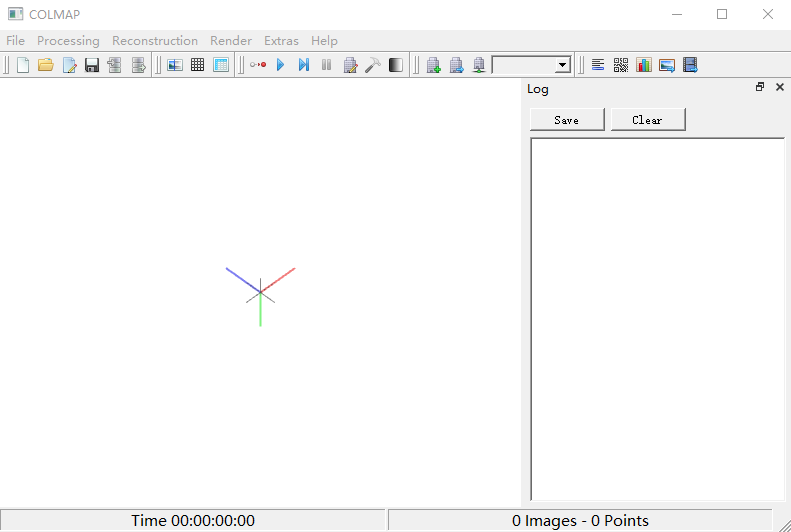
\includegraphics[width=14cm]{colmap-software}
	\caption{COLMAP软件界面}
	\label{colmap-software}
\end{figure}

\subsection{实验及结果}
本节中采用的数据集为在一个晴朗的午后于大礼堂南面使用单目相机拍摄的17张平面图像图片,分辨率为$1440\times 1080$像素,如图\ref{sfm-data}所示,分别编号为0-16。
\begin{figure}
	\centering
	\includegraphics[width=14.5cm]{SfM-data}
	\caption{大礼堂图像数据集}
	\label{sfm-data}
\end{figure}

采用windows10平台,COLMAP3.6无cuda加速版本软件,对以上17帧图像进行重建,其结果如图\ref{sfm-result}所示,其中红色四边形为相机成像平面的位置,其余点为利用SfM算法得到的大礼堂模型,结果中共有4121个点。
\begin{figure}
	\centering
	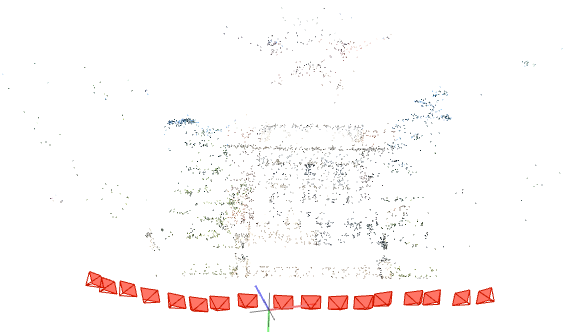
\includegraphics[width=14.5cm]{sfm-result}
	\caption{大礼堂场景SfM算法重建结果}
	\label{sfm-result}
\end{figure}

\section{基于激光雷达的LOAM三维重构}
\subsection{算法简介}
随着硬件水平的不断发展,激光雷达的尺寸和重量不断减少,这给基于激光雷达的定位建图技术提供了很好的基础;另一方面,激光雷达对于场景的探测不依赖于环境的光线条件与场景中的光学纹理信息,因此相比于基于视觉重建的SLAM算法,更适用于更暗场景的重建,同时也能带来更高的精度。

\citet{zhang2014loam}最早提出了以6DoF运动的两轴激光雷达进行场景重建的LOAM算法(Lidar Odometry and Mapping),图\ref{loam-pipeline}展示了这一算法的流程。$\hat{\mathcal{P}}$是当前通过雷达获得的扫描,$\hat{\mathcal{P}}$首先与之前$k-1$帧的点云的点云进行配准,得到$\mathcal{P}_k$。里程计模块通过比对相邻两帧的扫描来估计雷达的运动,同时纠正$\mathcal{P}_k$中的失真,该模块以1Hz的频率输出无失真的$\mathcal{P}_k$,以10Hz的频率对输出雷达的运动。前者经过Mapping模块将无失真的点云匹配并对其到已有地图上,最后结合这两者的变换,以10Hz频率输出最终的变换估计。
\begin{figure}
	\centering
	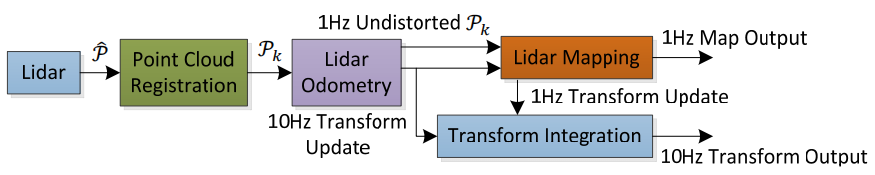
\includegraphics[width=14.5cm]{loam-pipeline}
	\caption{LOAM算法流程图}
	\label{loam-pipeline}
\end{figure}

为了更加高效地配准两帧扫描的点云,LOAM算法从每次扫描点当中选择两类点作为特征点。第一是角点,即位于扫描线上变化比较剧烈的点;第二类是平面点即线上曲率较小,变化缓慢的点。如图\ref{edge-plane-points}所示,对于角点,可以看做是位于真实世界中两个平面交线上的点,而对于平面点可以看做是真实世界中某一个平面上的点。LOAM算法通过优化当前帧角点到上一帧对应直线的距离和当前帧平面点到上一帧对应平面的距离,来进行位姿优化与运动估计。
\begin{figure}
	\centering
	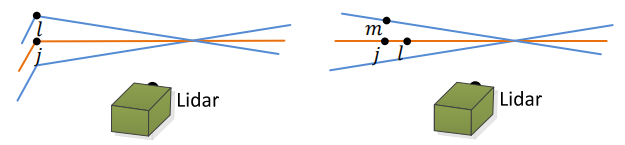
\includegraphics[width=12cm]{edge-plane-points}
	\caption{角点与平面点示意图}
	\label{edge-plane-points}
\end{figure}

\subsection{实验设备}
为了能更方便地在场景中实现控制和数据采集,本实验将一个移动运载底盘组装成小车系统,如图\ref{little-car},其最大速度为20km/h,即5.56m/s。
\begin{figure}
	\centering
	\subcaptionbox{实验小车\label{little-car}}
	{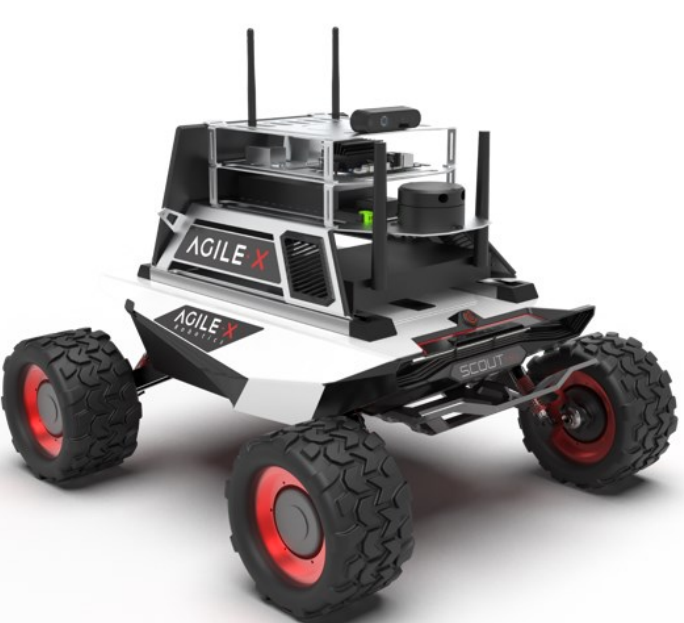
\includegraphics[width=6cm]{little-car}}
	\subcaptionbox{VLP-16激光雷达\label{vlp-16}}
	{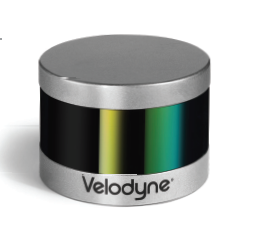
\includegraphics[width=6cm]{vlp-16}}
	\caption{实验设备}
	\label{loam-machine}
\end{figure}
同时在小车上搭载了16线激光雷达作为数据传感器,如图\ref{vlp-16}所示,能够实现$360^\circ$的在线扫描,其规格参数见表\ref{vlp-16-parameters}。
\begin{table}
	\centering
	\caption{VLP-16规格参数}
	\begin{tabular}{ll}
		\toprule
		指标 & 规格 \\
		\midrule
		测量距离 & 100m \\
		精确度 & +/- 3cm \\
		垂直视场角 & $+15^\circ$至$-15^\circ$ \\
		水平视场角 & $360^\circ$ \\
		垂直角分辨率 & $2^\circ$ \\
		水平角分辨率 & $0.1-0.4^\circ$ \\
		旋转速率 & 5-20Hz \\
		\bottomrule
	\end{tabular}
	\label{vlp-16-parameters}
\end{table}

\subsection{实验及结果}
利用上述设备,遥控小车在大礼堂门口的空地前走了一段距离,共拍摄300帧点云数据。利用LOAM算法生成了该区域的局部点云模型,结果如图\ref{loam-result}所示,其中白色的点云为重建结果,彩色的点云为激光雷达最后一帧的扫描数据,绿色线条为小车在地图中走过的轨迹。由于激光雷达扫描范围更广,并且相比于图像特征能够得到更多的点信息,因此局部重建结果更加稠密,在本次实验中,最终点云中共含有164145个点。
\begin{figure}
	\centering
	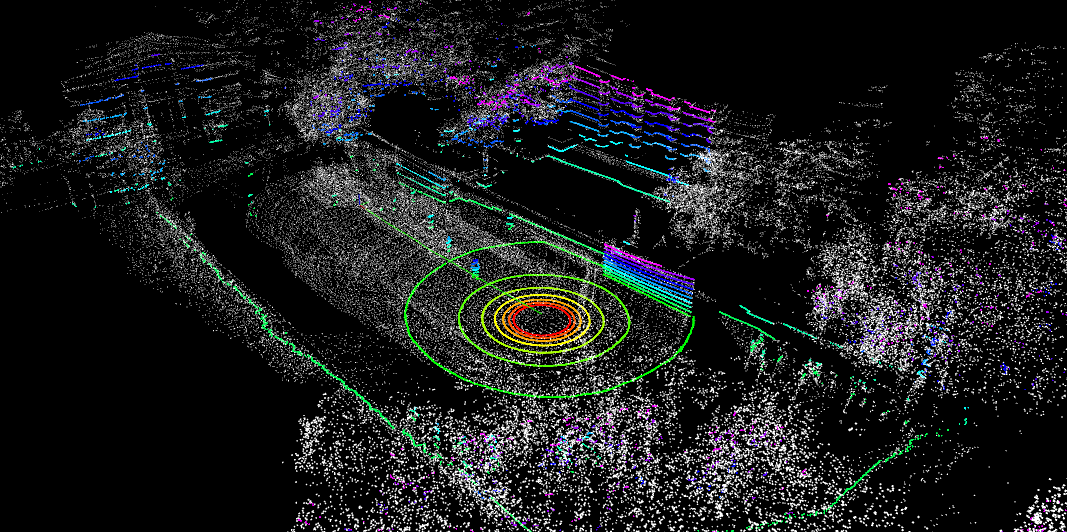
\includegraphics[width=13cm]{loam-result}
	\caption{大礼堂场景LOAM算法重建结果}
	\label{loam-result}
\end{figure}

\section{基于激光扫描仪的三维重构}
\subsection{Leica BLK360}
普通单目相机拍摄出来的照片,含有丰富的RGB颜色信息,但容易受到环境光照条件的影响;而采用普通激光雷达得到的数据,又由于只含有反射强度信息而缺乏颜色,因此含有的信息更少。而采用如图\ref{blk360}所示的激光扫描仪能够较好地平衡这两者的缺点,利用激光雷达与相机同时从环境中获取颜色与点云信息。
\begin{figure}
	\centering
	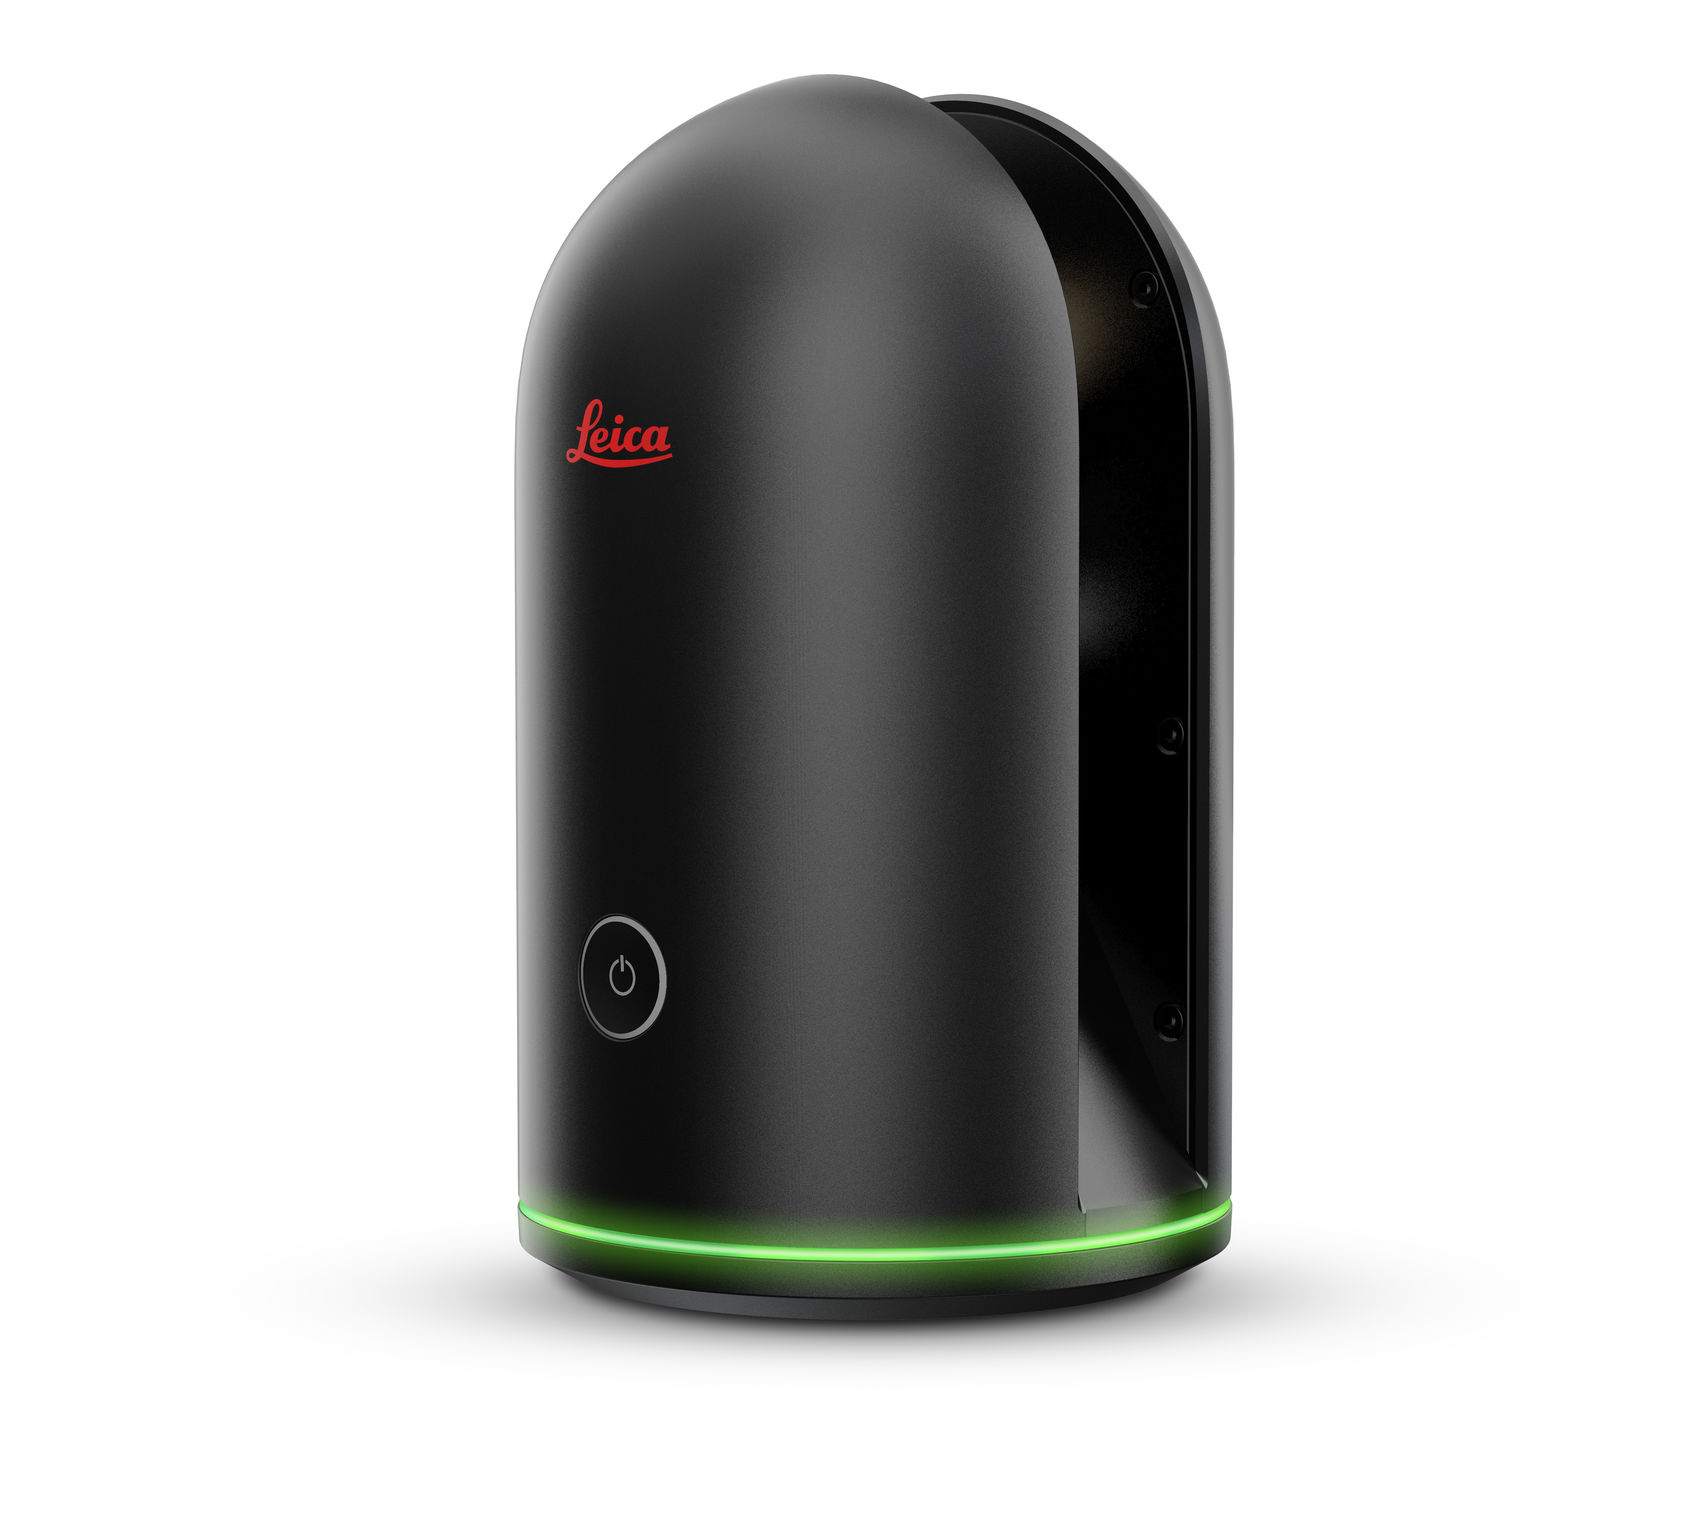
\includegraphics[width=6cm]{blk360}
	\caption{Leica BLK360激光扫描仪}
	\label{blk360}
\end{figure}

该设备的参数如表\ref{blk360-parameters}所示,相比于VLP-16,在一次扫描中它能够采集到数量更多、范围更广的点,但相应采集时间也更长,并且数据采集过程中要保证设备静止。
\begin{table}
	\centering
	\caption{Leica BLK360规格参数}
	\begin{tabular}{ll}
		\toprule
		指标 & 规格 \\
		\midrule
		测量距离 & 0.6-60m \\
		精确度 & 6mm @ 10m / 8mm @ 20m \\
		垂直视场角 & $+150^\circ$至$-150^\circ$ \\
		水平视场角 & $360^\circ$ \\
		分辨率 & 三级可调设置 \\
		扫描时间 & 3min \\
		\bottomrule
	\end{tabular}
	\label{blk360-parameters}
\end{table}

\subsection{扫描结果}
利用该扫描设备,以中等精度的分辨率,同样在大礼堂门口区域对其进行局部场景扫描。其结果如图\ref{blk360}所示,总共扫描得到6136121个点,各个点中包含了xyzrgb信息。
\begin{figure}
	\centering
	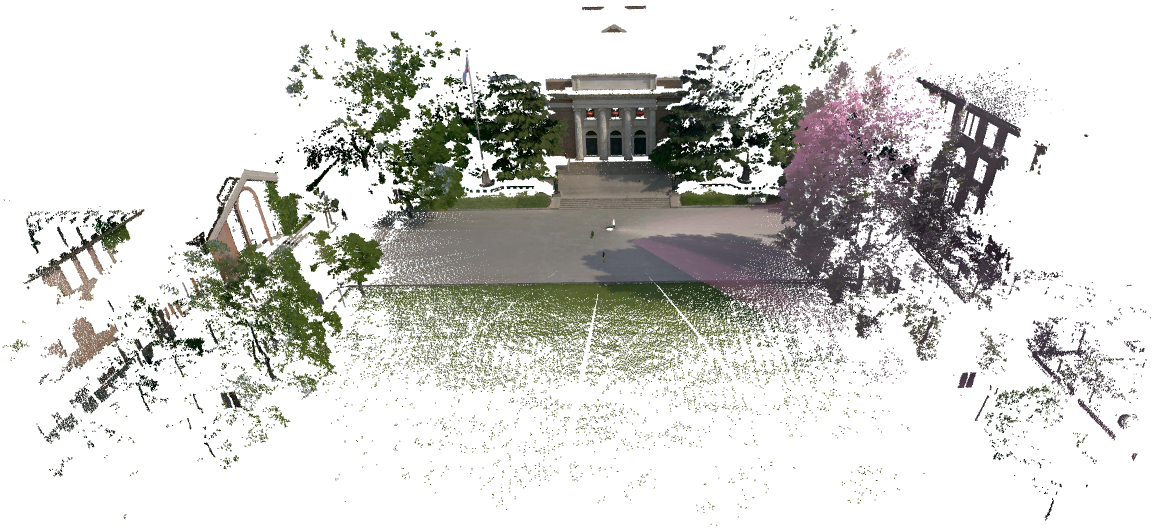
\includegraphics[width=14.5cm]{blk360-result}
	\caption{激光扫描仪重建结果}
	\label{blk360-result}
\end{figure}

\section{本章小结}
本章分别采用了纯视觉方法、纯激光雷达与基于视觉+激光雷达的方法,对于大场景中的局部区域进行了重建实验,实验结果表明,这三种采集设备与重建方式各具有优缺点,其汇总见表\ref{method-compare}。
\begin{table}
	\centering
	\caption{局部场景重建方法优缺点对比}
	\begin{tabular}{cccc}
		\toprule
		重建算法 & SfM & LOAM & 图像激光扫描法\\
		\midrule
		设备需求 & 单目相机 & 激光雷达 & Leica激光扫描仪 \\
		设备价格 & 便宜 & 较贵 & 昂贵 \\
		采集时间 & 较短 & 较短 & 长 \\
		重建时间 & 长 & 较短 & 无需额外重建算法 \\
		重建精度 & 稀疏 & 一般 & 稠密 \\
		\bottomrule
	\end{tabular}
	\label{method-compare}
\end{table}

对于SfM算法而言,其最大的优点就是设备价格便宜,仅需使用单目相机就可以完成,并且采集成本较低,仅需对场景的不同角度进行拍照即可完成,但同时带来的代价是重建时间较长,因为特征的匹配搜索需要耗费大量的资源,并且重建精度较低;对于LOAM算法而言,其采用的激光雷达设备较为昂贵,但数据采集方便,仅需遥控小车即可完成,同时能够实时地完成地图构建任务;对于图像激光扫描法而言,其优点在于得到的点云非常稠密,并且不需要进行额外算法即可得到局部的点云数据,其缺点在于设备昂贵,并且数据采集的时间成本较高。

因此,在实际的局部重建中,需要根据成本及精度要求,选择合适的算法。